\textbf{\LARGE{Part one: Design Project}}
\todo[inline]{Part one is a design project report as described
    in the coursebook. The audience for this is the companies
    management. See e.g.\ page 186ff.
    Length between 25-30pp}

\section{Objective}

\subsection{Objective of the design project}
The focus of the design project is to improve upon the booking process used by 
\gomonkey. The booking process is currently very manual and only ever handled by 
the manager. The manager said that: 

\begin{quotation}
I don't dare letting my employees handle the bookings!

\em - Michel Pascual, manager and owner of \gomonkey{}, 15.10.2013
\end{quotation}

He is afraid they will make mistakes, since the process is complex and not very 
well documented. Some bookings may also contain cases which the manager is not 
yet sure of how should be handled, and thus needs an authority to handle and  
produce a best practice for \gomonkey{}. While the manager does spend a lot of
time handling bookings, this takes time from actually evolving the business.
The goal of the design project is to put the booking process into a 
well defined system and reduce the complexity and time required for handling
incoming bookings. This will reduce the workload put on the manager, thus 
empowering him to focus on other areas of the business.

\subsection{Results from the in-line analysis}
The in-line analysis is meant to help us understand the environment in which 
the company is situated, the business strategy of the company, and what work
domains are defined within the business. This will help the designers to
better understand the reasoning behind current work practices and how to 
solve the problems that arise. The most noteable parts of the results from 
the in-line analysis are the business strategy and the overview of the work 
domains of \gomonkey{}.

\subsubsection{Business strategy}
The business strategy of \gomonkey{} was not written down before we started the
project, so we had to construct and interpret on our perception of the company.
This changed during the course of the design project, and this is the final 
result:

\begin{enumerate}
	\item Become a self-sustainable climbing company with customers on a daily basis.
	\item Minimize time requirements pr.\ booking/customer.
	\item Minimize staff requirements to keep costs low.
	\item Increase sales (Such as selling food, drinks, etc.).
	\item Provide better and more comprehensive services than competitors.
\end{enumerate}

While these are not easily quantifiable, and thus are not a very suitable list
for a business strategy, it will work for this purpose. Whenever we do suggest
a change for the company, we should be able to, directly or indirectly, point to
a specific point in the business strategy.

\subsubsection{Work domains}
The company, while selling climbing sessions as a service, clearly does other
things that does not directly add value, but a necessary nonetheless.		%this is spelled correctly! nonetheless
While interviewing and observing the company, we mapped out those areas of 
work, and the result can be seen in \autoref{table:workdomain}.

\begin{table}[H]
    \centering
\begin{tabular}{ |l|l| }
        \hline
        Work domain & Example work processes \\ \hline
        \multirow{4}{*}{Booking Flow} 
            & Registering received bookings \\
            & Checking payment status \\
            & Informing customers prior to arrival \\
            & Receiving customers \\
        \hline
        \multirow{3}{*}{Employee Schedule} 
            & Scheduling shifts \\
            & Swapping shifts \\
            & Time registration \\
        \hline
        \multirow{2}{*}{Economy and bookkeeping} 
            & Payment during booking \\
            & Invoice after visit \\
        \hline
        \multirow{2}{*}{Inventory Management} 
            & Maintenance of inventory \\
            & Stock control of equipment \\
        \hline
        \multirow{2}{*}{Marketing} 
            & Advertising \\
            & Offers and discounts \\
        \hline
\end{tabular}
\caption{List of work domains and example work processes in the specific work domain}
\label{table:workdomain}
\end{table}

This makes us more aware of what the company does. This can be used to further 
explore what processes exists and map exactly how they are performed. But more 
important, this allows us to ignore certain parts of the company that are not 
related to the problems we are trying to solve with a system. An effort focused
on a single work domain is bound to get into more details, and thus yield a 
better result.


\subsection{Results from the in-depth analysis}
\todo[inline]{Observations, standard systems, work practices}

The in-depth analysis is meant to help us understand exactly how and why the 
existing processes work as they do. This was done by observing the processes,
analysing documents and correspondance, and mapping out exactly what work 
practices resulted in problematic situations. In the following section we describe the 
work practies we found, and what problems were discovered. When we knew the
business practices and related problemss, we surveyed the market for a useable 
standard system, which is described later in this section.

\subsubsection{Work practices and their problems}

\subsubsection{Finding a suitable standard systems}
It is often a good solution to find a standard system which solves the problem 
at hand. This can save a lot of time and money, and can quickly solve a complex
problem.
We compiled a list of possible standard systems and isolated three very possible
candidates. After deep testing sessions of all systems, we realized that none
of them fulfill the defined requirements in the design project. The testing
session included creating a free temporary booking system. All systems tend to 
have this feature, so potential customers can evaluate the usefullness prior to 
paying. Attempts were then made to setup the system to support the needs of
\gomonkey{}, and after testing the usefullness of the result, we could conclude
upon the advantages and disadvantages of implementing the system.

\begin{description}
\item[SuperSaaS]
We decided not to use SuperSaaS, since the booking doesn’t support the required 
fields for the booking. A `form' can be attached to a booking after submitting 
initial information (intial information being the date and time of booking, 
name, phone number and email address), and this 
form can include extra information about amount of people in each age group, the
type of customer and food. This information can only be seen with two clicks 
from the calendar overview, thus making it impossible to get a good overview of 
how `available' a time slot is.

Furthermore, it is not possible to calculate a price based on the custom fields 
in the form, and as such, the system cannot ask for a deposit so we will still 
need another payment processor.

\item[onlinebooq.dk]
The second promising booking system was onlinebooq.dk. They support selling 
`services', but unfortunately they only support selling one of each servive.
This can be seen in \autoref{fig:onlinebooq} as the checkbox, next to the 
service in question. This makes it useless for \gomonkey{}, since the price is 
calculated from the amount of people utilizing each service. It does support 
paypal and quickpay, but this doesn't matter if we cannot calculate the price 
correctly.

\begin{figure}[htbp]
    \centering
        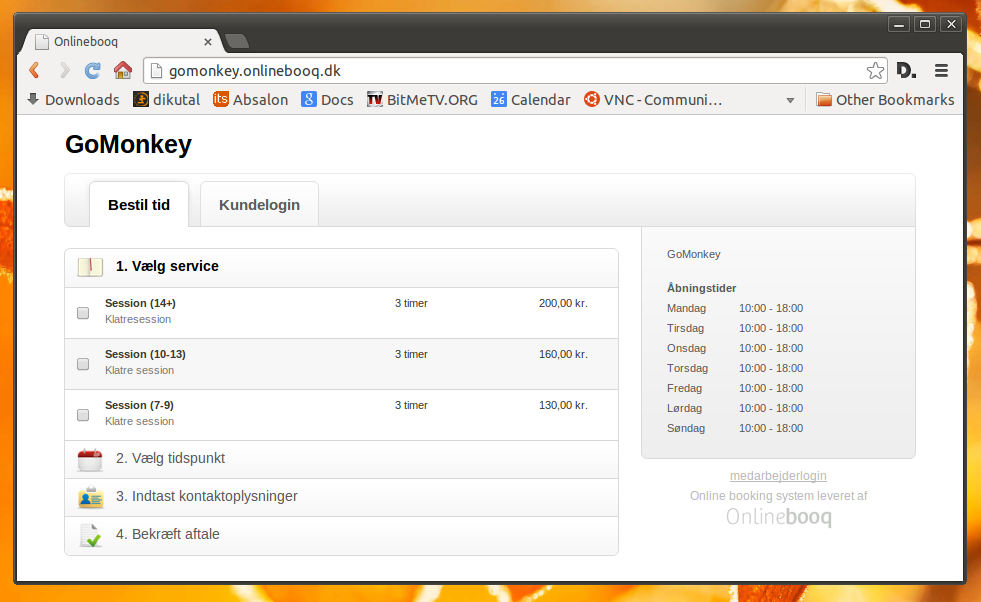
\includegraphics[width=.8\textwidth]{figures/onlinebooq.png}
	    \caption{Screenshot from testing onlinebooq.dk.}
        \label{fig:onlinebooq}
\end{figure}
		

\item[Cyberbooking]
The last booking system we tested was Cyberbooking. They have two types of 
calendars, one which supports one resource (e.g.\ a hairdresser) who can only
perform one service at a time. The other type supports booking slots on 
predefined events, (e.g.\ a fitness session) and the events are set by the 
company. None of these types can help \gomonkey{} with the booking process,
since the amount of resources aren't limited to one group of customers, and 
the times of bookings are very flexible.
\end{description}

While none of the systems fit with \gomonkey{}'s business, we attempted
to find a way to adjust \gomonkey{}'s business to the systems. This was not 
successful and would alter the work practices in a very negative way.

\newpage
\section{The coherent vision}
The coherent vision we suggest here is based on the results from the in-line 
analysis and in-depth analysis. The vision is a suggestion for a system design, 
along with descriptions of any expected organizational additions and changes 
resulting from implemeting the system. It also includes reflections upon 
required qualifications of anyone who will have to interact with the system
and what advantages and disadvantages this will enforce thoughout the company.
Finally, it includes some financial figures and an implementation plan. This 
should give the required knowledge of the system to perform an informed choice
on wether to start the project.

\subsection{Technology and systems}
This section will describe the system itself, what it does and how it looks,
along with what is required to keep the system running. This is intended to 
help building the system, should the project be initiated.

\subsubsection{IT systems and platform}
The owner of \gomonkey{} insists that the main website continues to run on the 
WordPress which is hosted with One.com. This is a fine solution, and will make
sure that the website maintains it's current, existing Google page-rank.

Further, it is necessary to have a server for hosting the new system, with 
access to a database and a webserver. This is not achievable on the server from 
One.com, so another will have to be found. It will be sufficient to have 
interfaces to a database and a webserver, but it is optimal to have root acess
to the server.

The server can run any operating system which supports a database and a 
webserver, but preferably a free one, to avoid the costs of the license for a 
proprietary system.

Additionally, there will still be parts of the original system which remain. 
The scheduling and journaling of staff will still be hosted in the company's 
Google Drive. 

\subsubsection{Components, functions and interface}
The system contains 5 general components;
\begin{itemize}
\item Booking form
\item Booking status page
\item Administrative overview
\item Administrative booking status
\item Todays bookings
\end{itemize}

The bare \textbf{booking form component} can be seen in \autoref{fig:bookinitial}. The booking
form incorporates many of the original features and functions of the existing 
\gomonkey booking form. The user is expected to input values for a number of 
different fields:
\begin{enumerate}
	\item Name or Company (Text string)
	\item E-mail address (Text string)
	\item Phone number (Text string)
	\item Day of booking (Calendar-valid date found with a calendar widget)
	\item Starting time (Valid 24h-format time)
	\item 0 or more participants between age 7-9, age 10-13 and age 14+, at minimum 1 participant.
	\item How the user heard of GoMonkey (Radio box)
	\item Optionally, food and drink can be ordered as well.
\end{enumerate}

A price calculator has been added as part of the booking form, that provides 
a running total of the cost of the booking as well as any deposit, if the cost
of the booking is large enough. A Frequently Asked Questions section has been 
moved directly into the booking form, for easy viewing during booking.

An example of a filled booking page can be seen in \autoref{fig:bookfilled}. The
'Submit' button will prepare the booking, for a final view for the customer to 
check that the information are correct. This can be seen on 
\autoref{fig:bookconfirm}. If the user agrees to the entered information, the
user can click 'Book' and the booking will be sent while the user is presented
with a modal popup that informs the user that the booking will need to be confirmed,
and that there might be a required deposit. This can be seen on 
\autoref{fig:bookconfirmpressed}.

\begin{figure}[htbp]
    \centering
        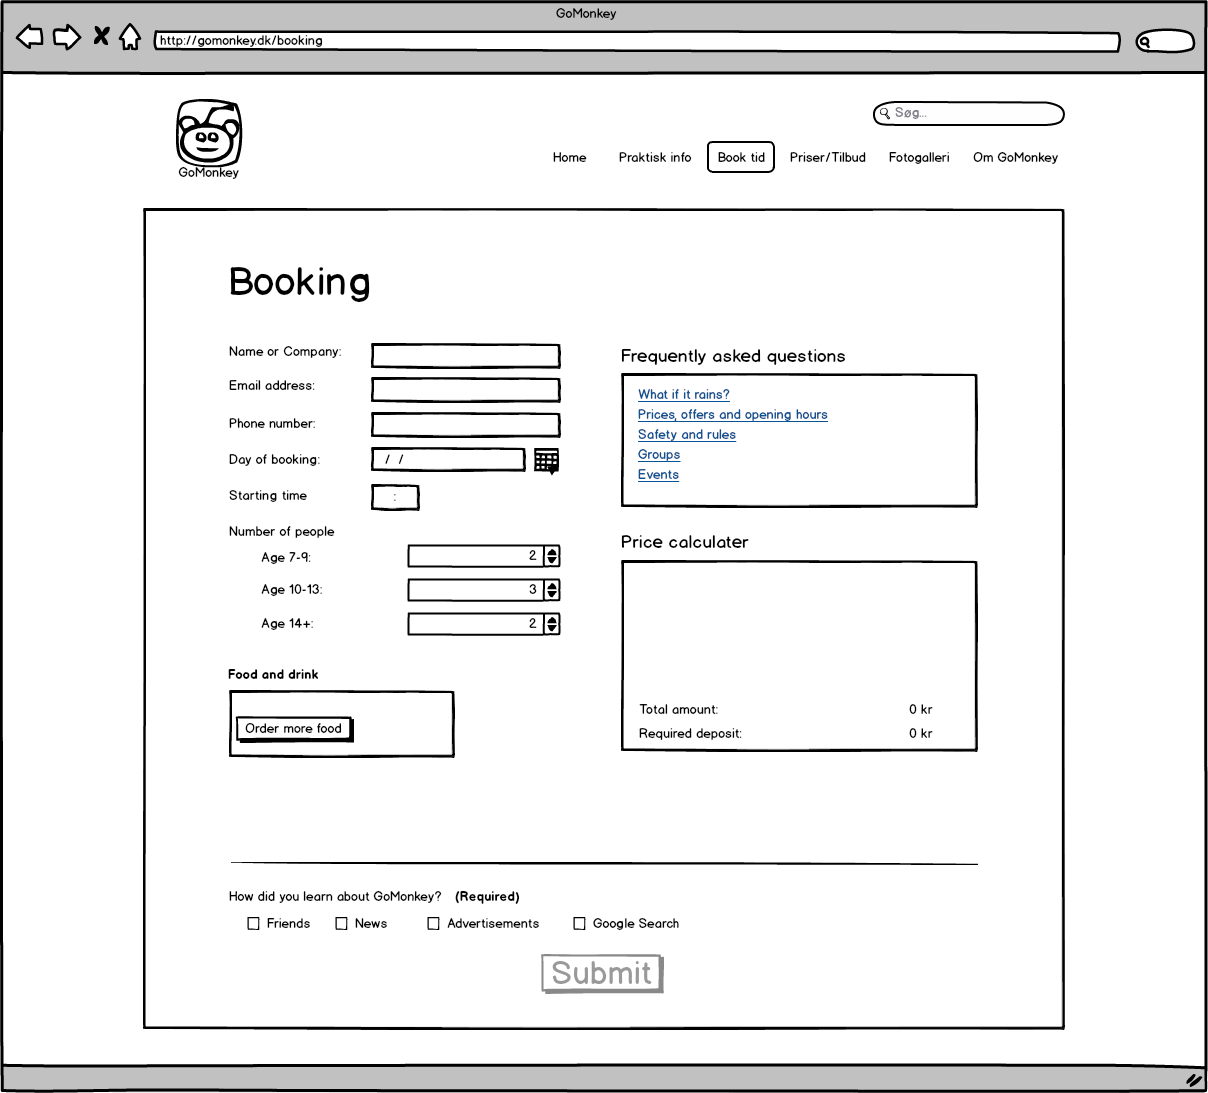
\includegraphics[width=.8\textwidth]{figures/mockup/booking_initial.png}
	    \caption{The bare booking form which the customers will find on the WordPress website.}
        \label{fig:bookinitial}
\end{figure}
\begin{figure}[htbp]
    \centering
        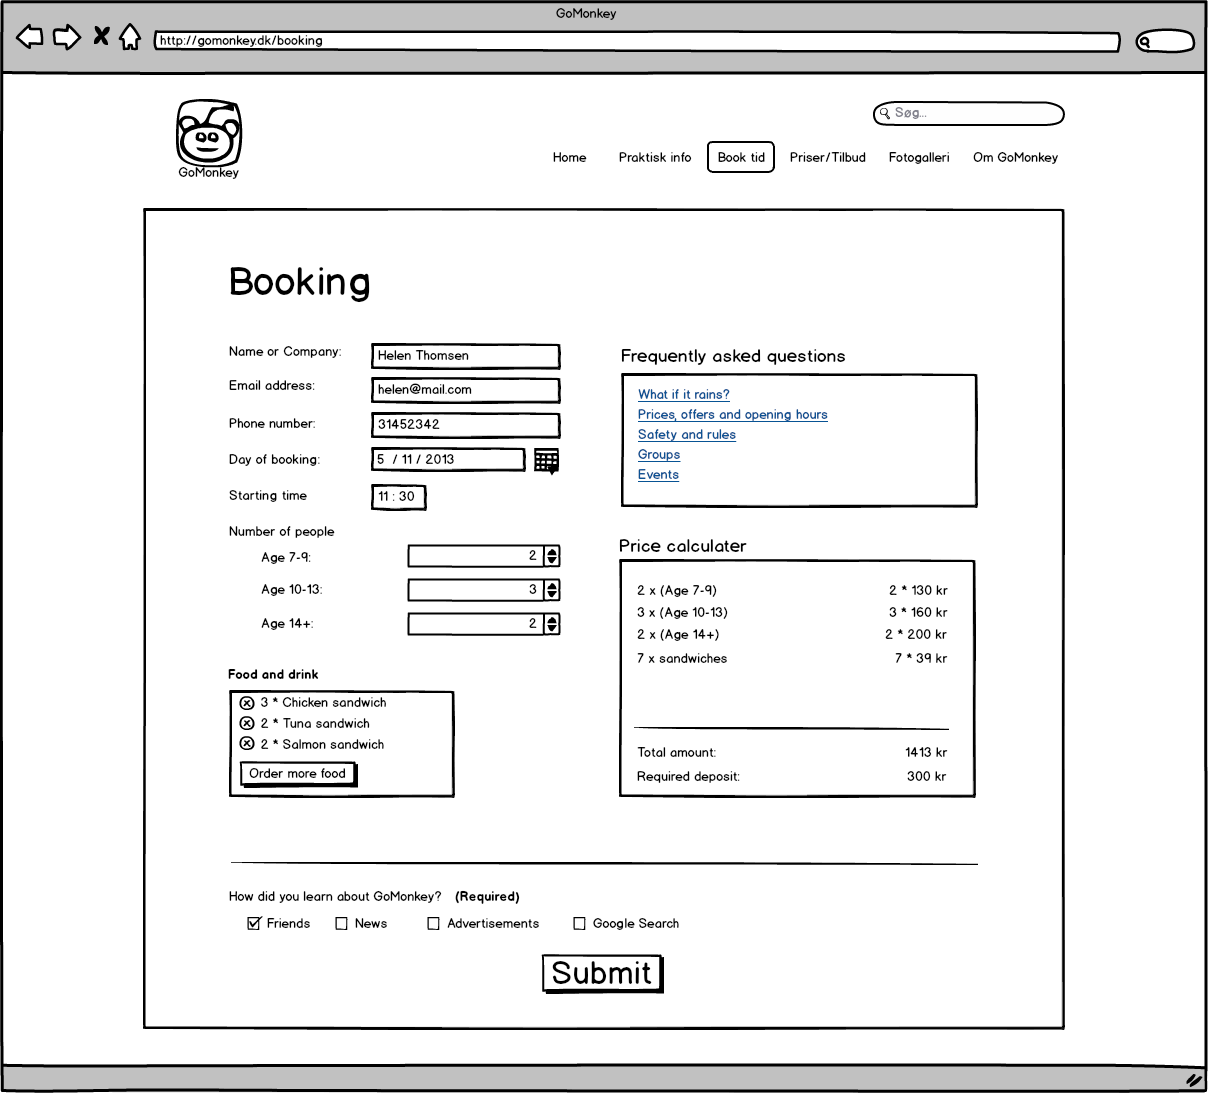
\includegraphics[width=.8\textwidth]{figures/mockup/booking_filled.png}
	    \caption{The booking form is filled and ready to be submitted.}
        \label{fig:bookfilled}
\end{figure}
\begin{figure}[htbp]
    \centering
        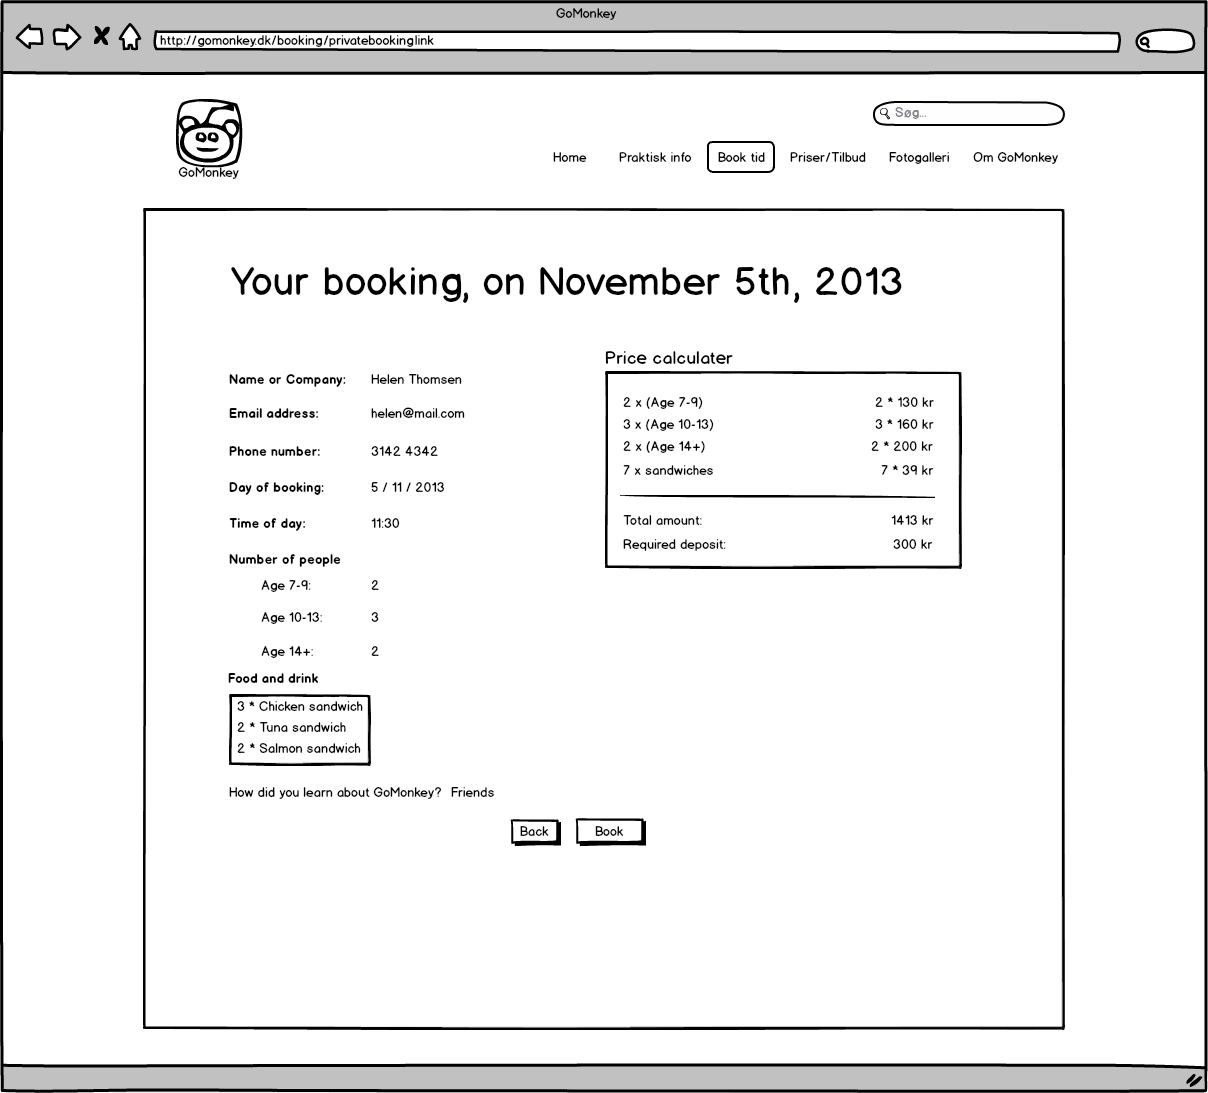
\includegraphics[width=.8\textwidth]{figures/mockup/booking_confirmation.png}
	    \caption{The booking form is submitted and the customer can view the entered information before finally booking.}
        \label{fig:bookconfirm}
\end{figure}
\begin{figure}[htbp]
    \centering
        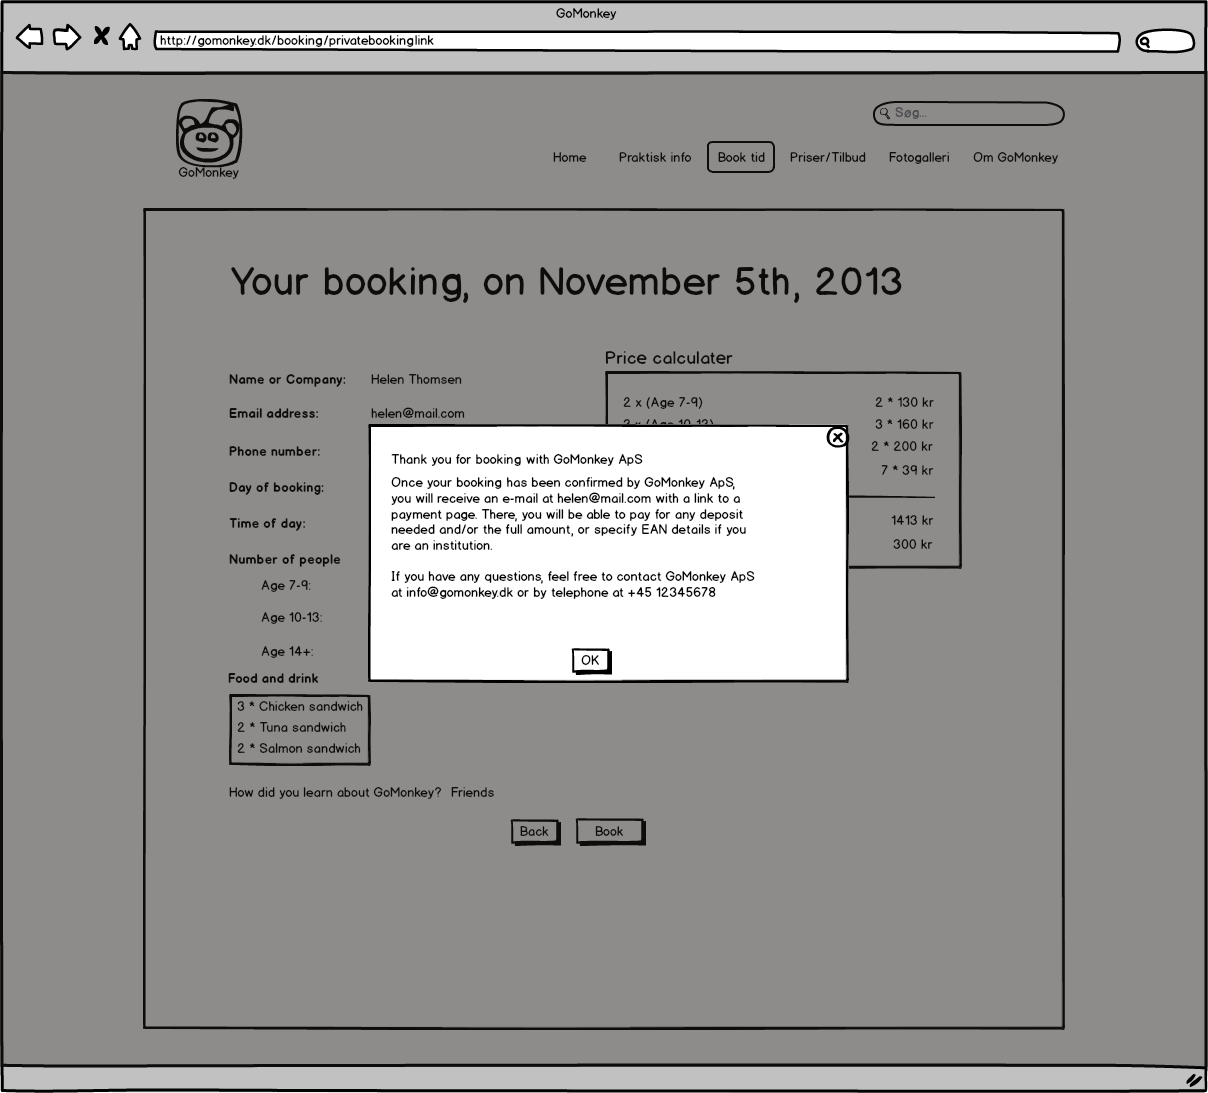
\includegraphics[width=.8\textwidth]{figures/mockup/booking_confirmation_bookpressed.png}
	    \caption{The booking form is submitted and the customer is informed about the following process.}
        \label{fig:bookconfirmpressed}
\end{figure}

The \textbf{booking status component} on \autoref{fig:bookstatus1} looks quite similar 
to the booking form, but the 
user cannot make any changes to the booking. In addition to a list of all of 
the things the user could see in the Booking form, the user can also see 
whether \gomonkey{} has confirmed the booking or not and can pay for the deposit 
and/or the full cost of the booking.

An unconfirmed booking can not yet be paid for in any way. However, once a 
booking is confirmed by \gomonkey{} the payment options appear, as in 
\autoref{fig:bookstatus2}. Payment occurs 
by clicking on either a ‘Pay Deposit’ button, or a ‘Pay full amount’ button. 
For institutions, there is also a ‘Confirm payment via EAN’ button, which 
allows the user to enter EAN-related details instead.

Finally, when an amount has been selected, is is possible to select a preferred
payment processor, as in \autoref{fig:bookstatus3}. This is important, since 
instant online transactions are very
critical to the function of the system.

\begin{figure}[htbp]
    \centering
        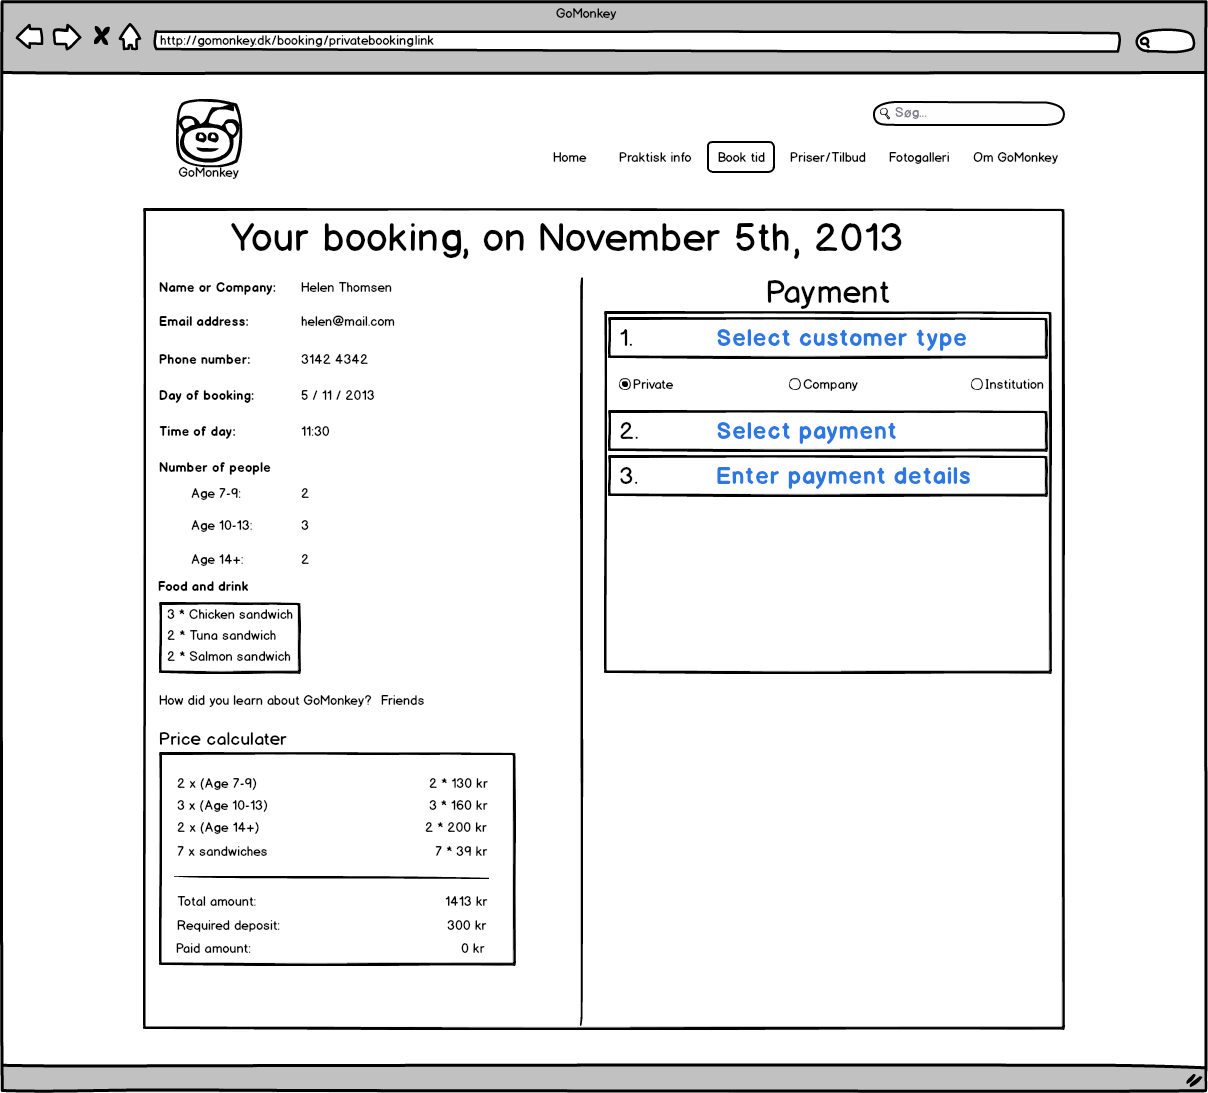
\includegraphics[width=.8\textwidth]{figures/mockup/booking_payment_1.png}
	    \caption{The customer can see the booking, but can't pay until the date and time has been confirmed.}
        \label{fig:bookstatus1}
\end{figure}
\begin{figure}[htbp]
    \centering
        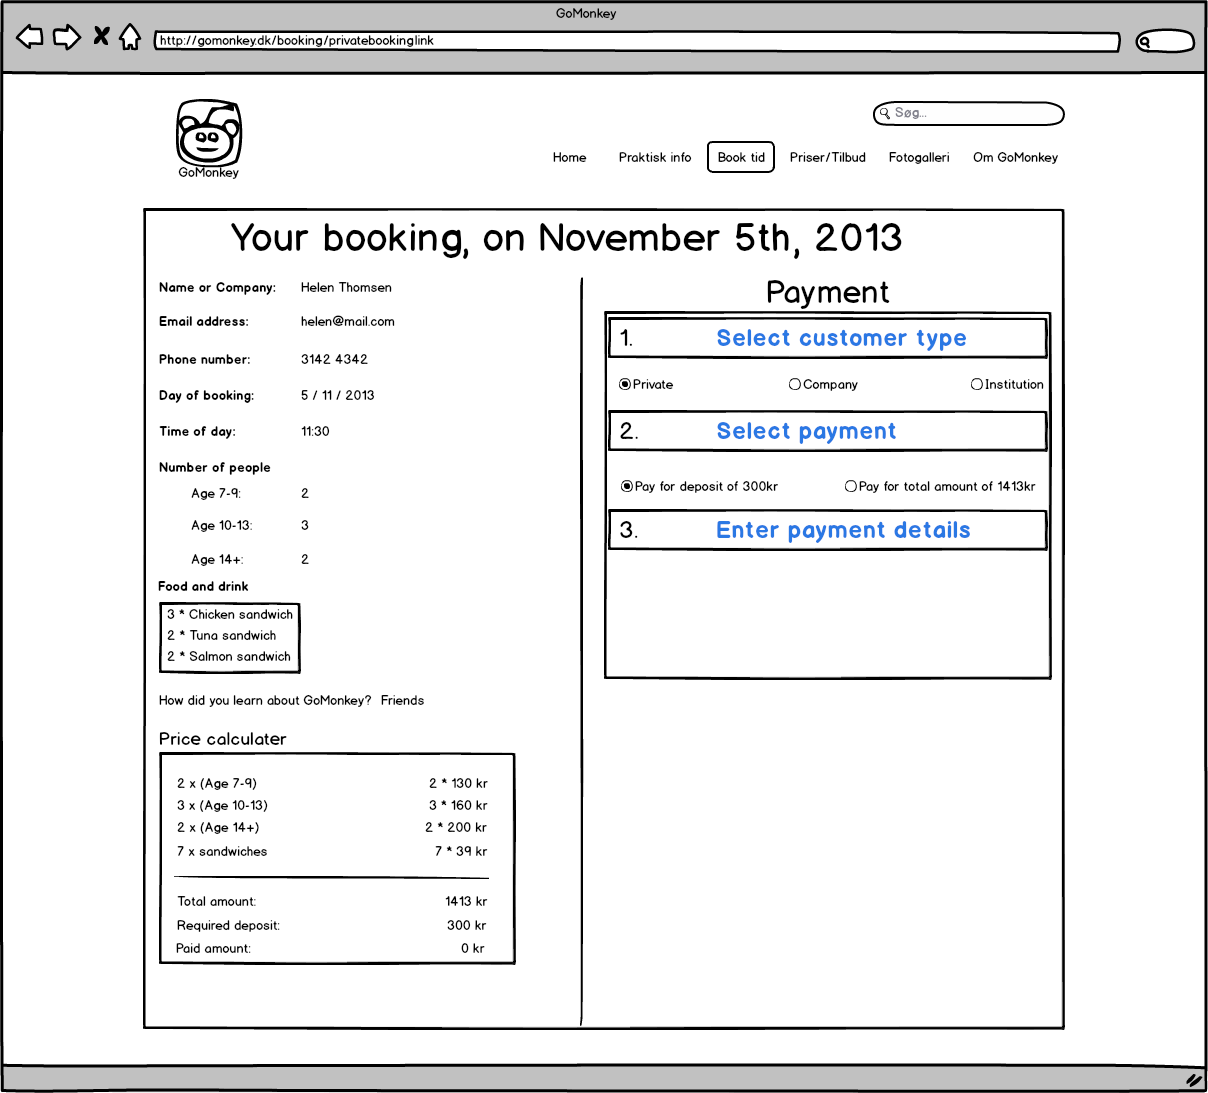
\includegraphics[width=.8\textwidth]{figures/mockup/booking_payment_2.png}
	    \caption{The customer is now able to select the desired amount to be paid, prior to visiting the park.}
        \label{fig:bookstatus2}
\end{figure}
\begin{figure}[htbp]
    \centering
        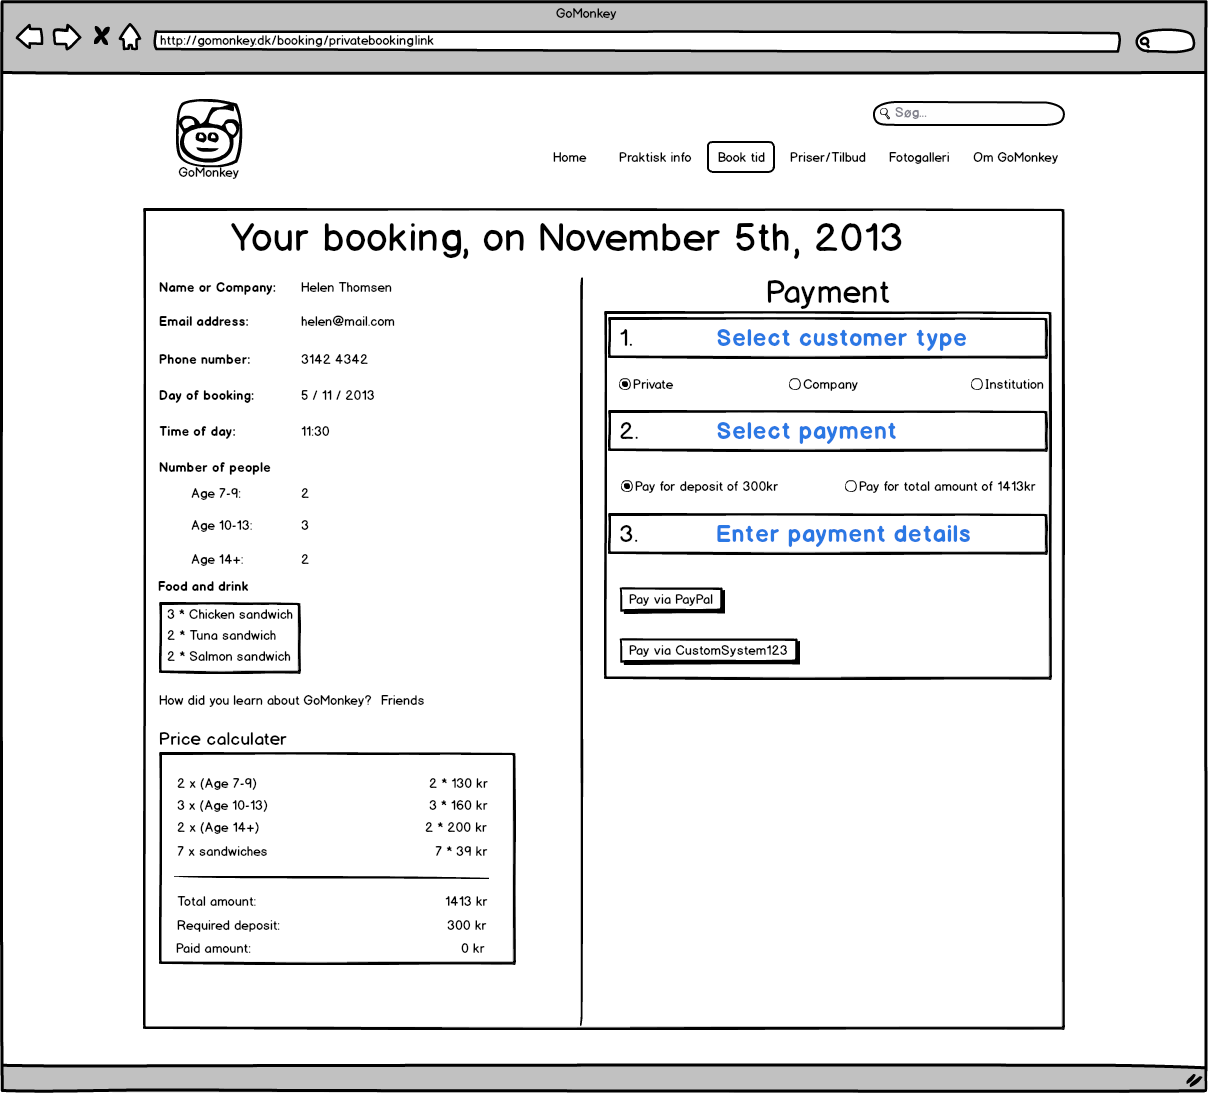
\includegraphics[width=.8\textwidth]{figures/mockup/booking_payment_3.png}
	    \caption{Finally, the customer can select a preferred payment processor and pay instantly.}
        \label{fig:bookstatus3}
\end{figure}

The \textbf{administrative overview component} displays the incoming bookings which require an 
action from the manager, and can be seen in \autoref{fig:adminoverview}. The 
date, time and amount of people is shown for quick confirmation, and is needed,
each booking can be entered and scrutinized with the administrative booking status.

\begin{figure}[htbp]
    \centering
        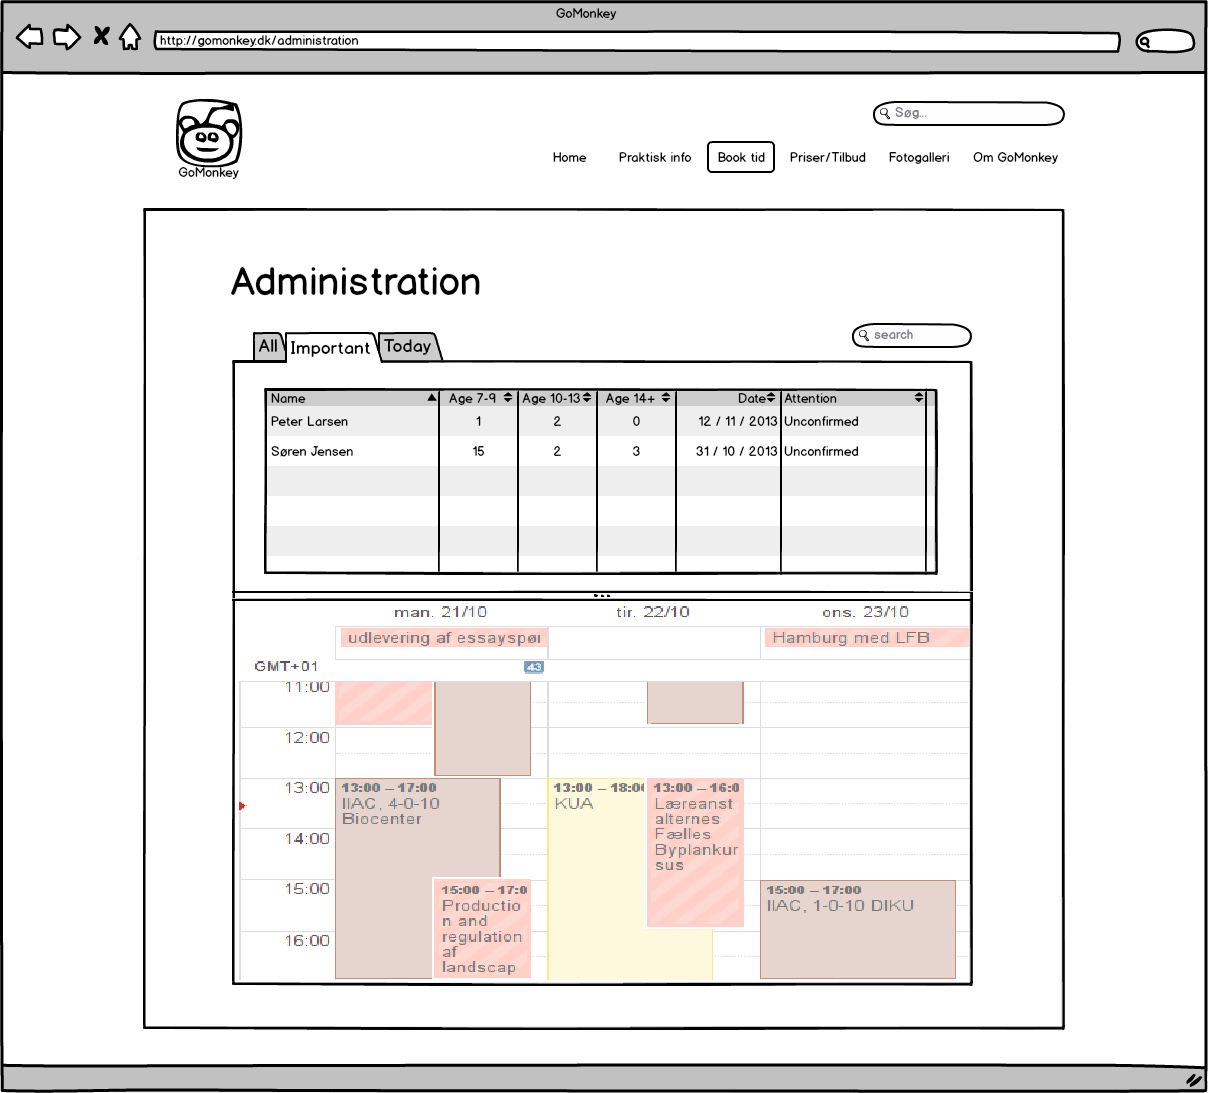
\includegraphics[width=.8\textwidth]{figures/mockup/overview_important.png}
	    \caption{The manager get a good overview of the incoming bookings which requires an action.}
        \label{fig:adminoverview}
\end{figure}

The \textbf{adminstrative booking status component} describes a booking in full and allows the
\gomonkey{} manager to either confirm a booking or decline it, based on the 
calendar overview presented next to the confirmation box. This can be seen in
\autoref{fig:admin}. 

If the manager accepts a booking, an e-mail will be sent to the user notifying 
them of this, and the user-viewable booking status page will reflect that the 
booking has been accepted. The booking is now open for the user to pay 
deposit/full amount. This can be seen in \autoref{fig:adminconfirmed}.

If the manager declines a booking, an e-mail will be sent to the user notifying 
them of this, and the user-viewable booking status page will reflect that the 
booking has been declined. The manager can supply a reason at the time of 
declining, with either a standard response, or a manual response with a
suggested alternative time and date. This can be seen in \autoref{fig:admindecline}

\begin{figure}[htbp]
    \centering
        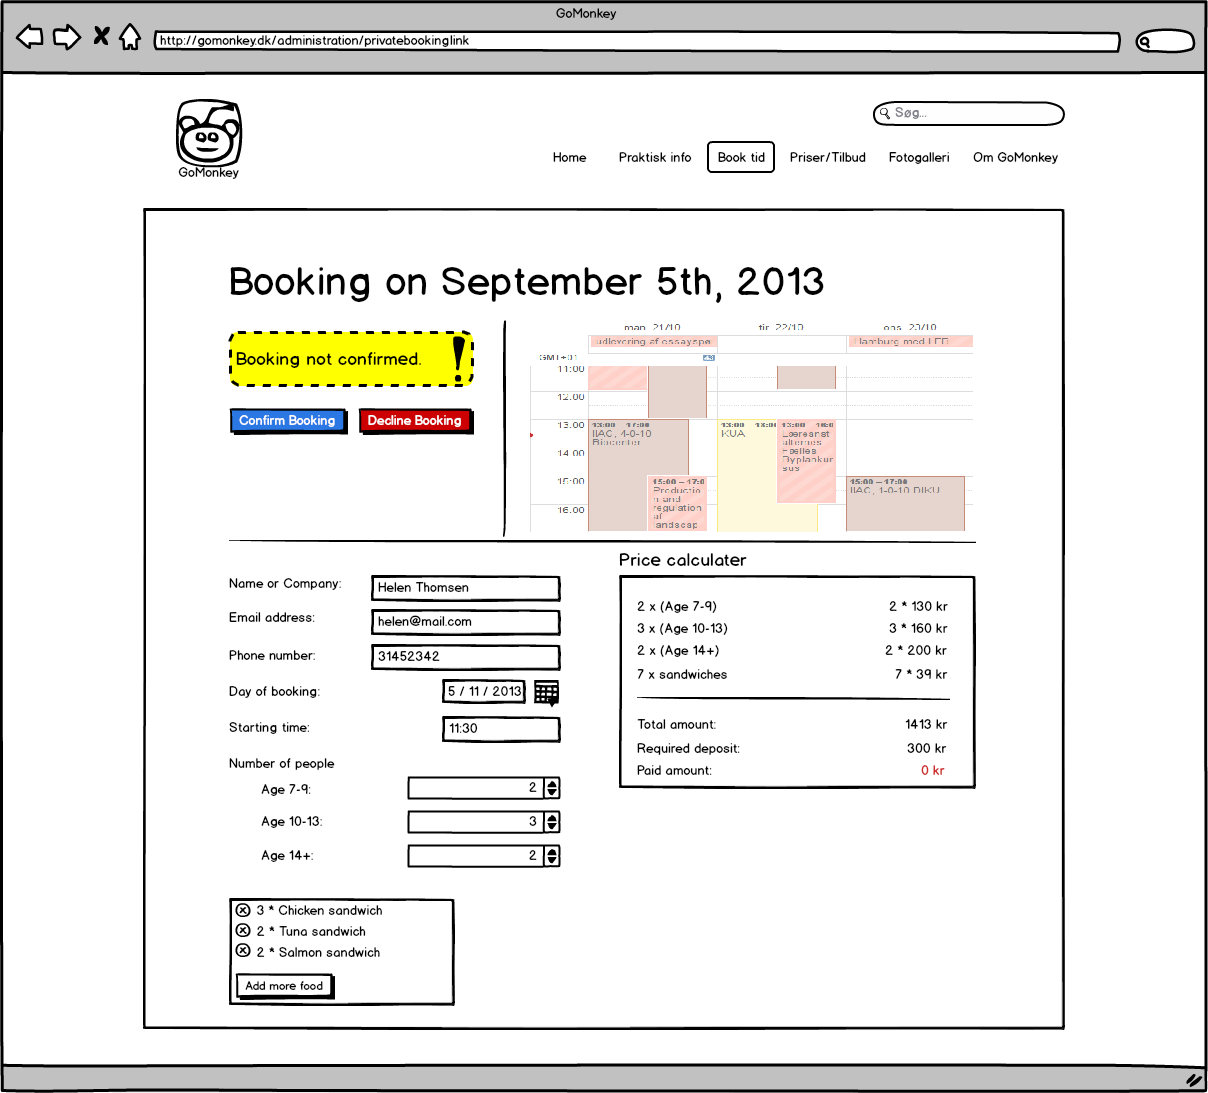
\includegraphics[width=.8\textwidth]{figures/mockup/admin_booking.png}
	    \caption{The manager can view the booking and see the calendar dates surrounding the booking.}
        \label{fig:admin}
\end{figure}
\begin{figure}[htbp]
    \centering
        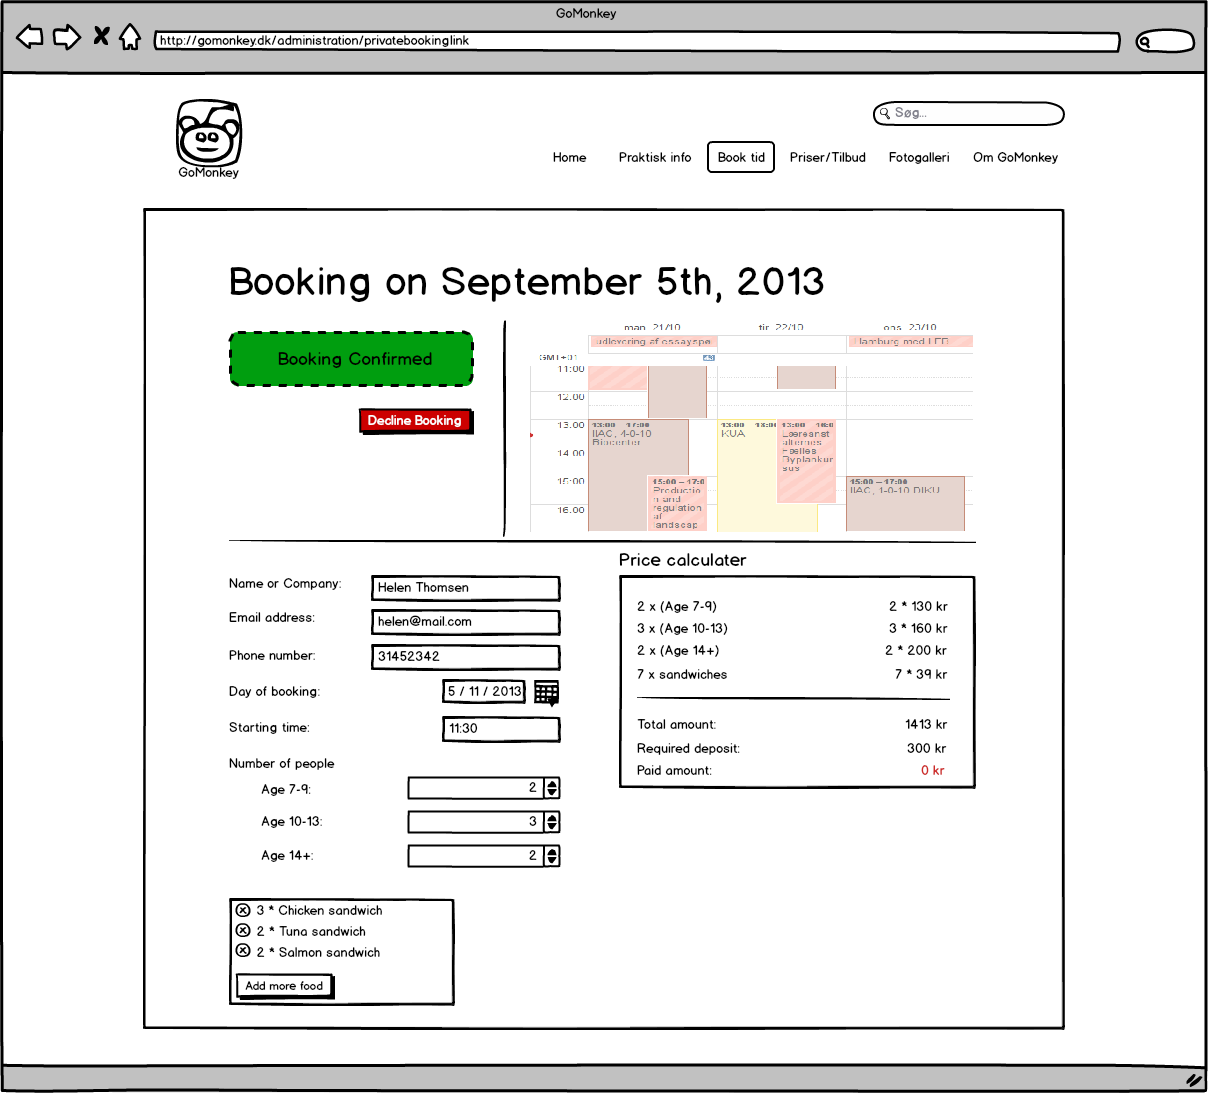
\includegraphics[width=.8\textwidth]{figures/mockup/admin_booking_confirmed.png}
	    \caption{The manager has confirmed and the customer can now pay for the session.}
        \label{fig:adminconfirmed}
\end{figure}
\begin{figure}[htbp]
    \centering
        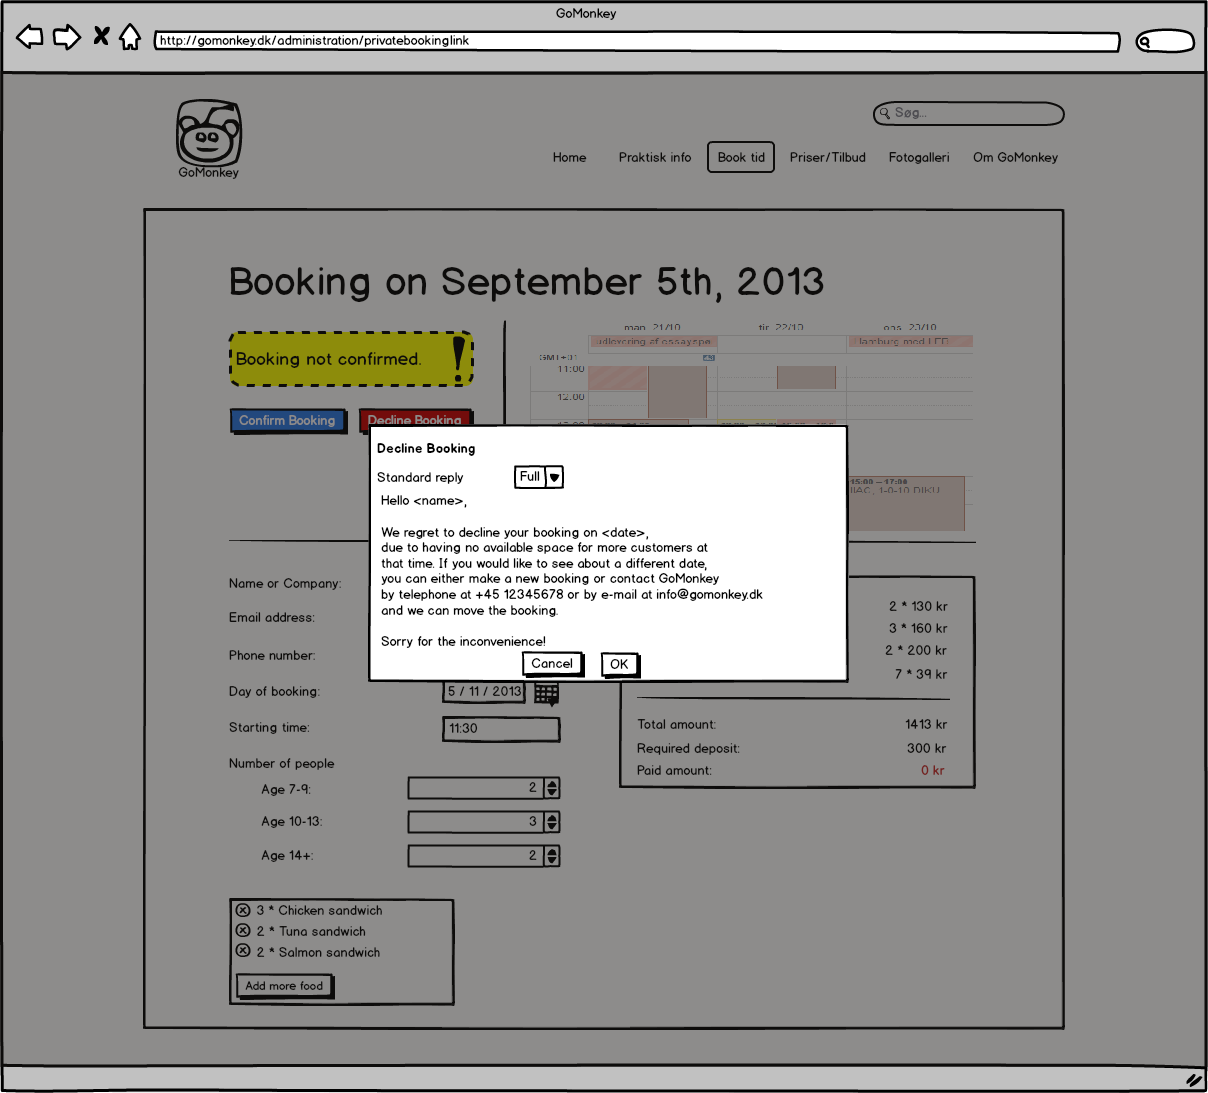
\includegraphics[width=.8\textwidth]{figures/mockup/admin_booking_decline.png}
	    \caption{The manager can decline the booking with a message describing why he had to decline, or attach a custom message.}
        \label{fig:admindecline}
\end{figure}

The final component is the \textbf{overview of todays bookings} and can be seen in
\autoref{fig:overviewtoday}. This is intended for 
the instructor to get a quick overview of how many people are coming on the 
day, when they will come, and how much they will need to pay, and whether
they ordered something extra. This will help the instructor handling booked 
groups. Especially if there is a booking for a big group, the instructor will
know not to take big groups just prior to having the booked group arrive.

\begin{figure}[htbp]
    \centering
        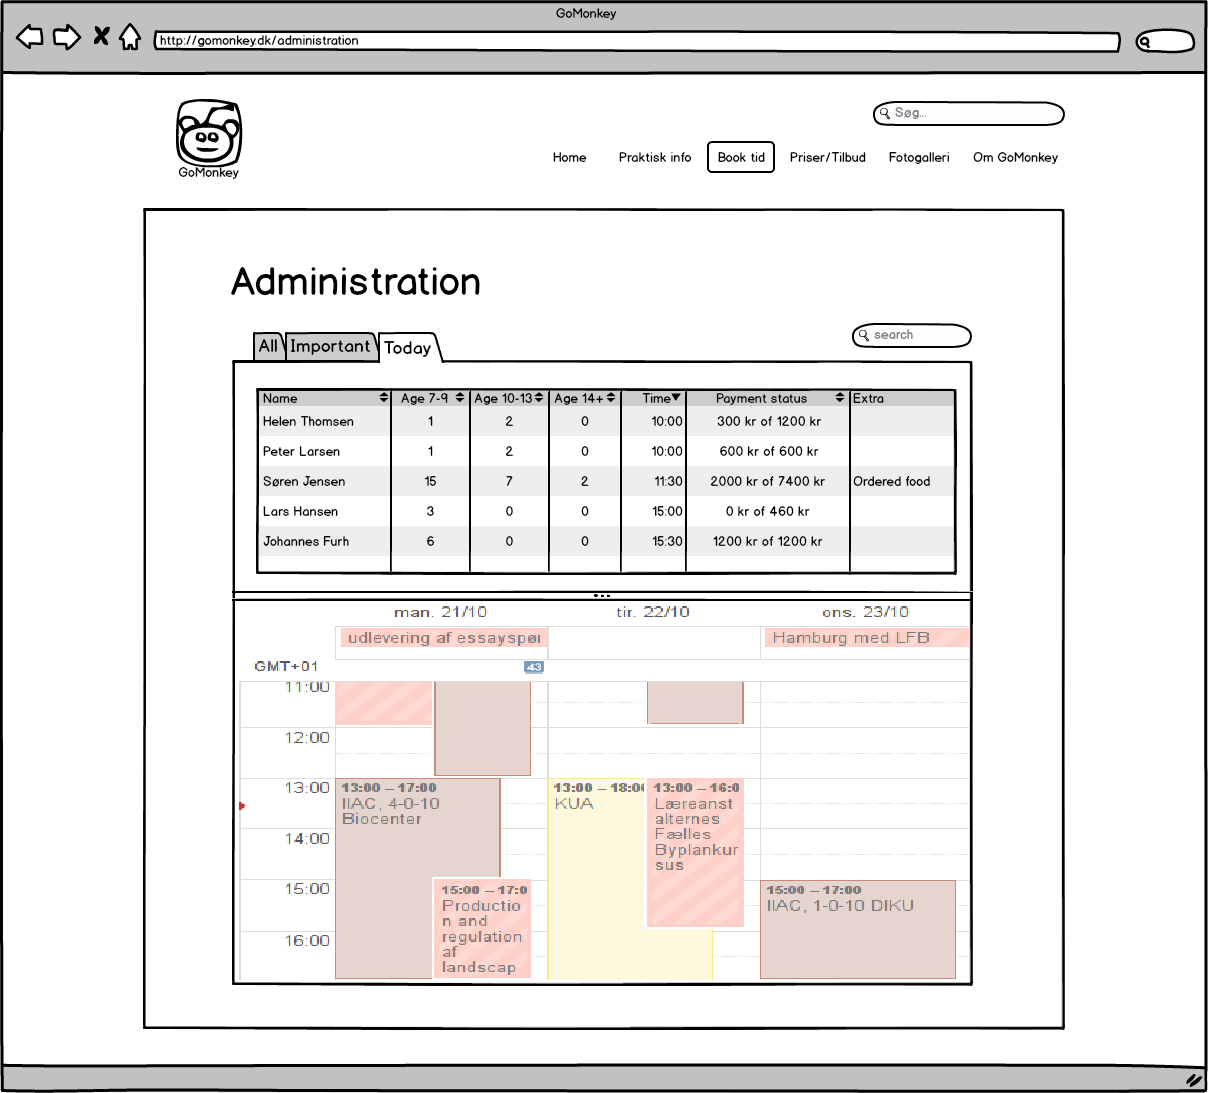
\includegraphics[width=.8\textwidth]{figures/mockup/overview_today.png}
	    \caption{The instructor can easily see what times there will be incoming groups.}
        \label{fig:overviewtoday}
\end{figure}


\subsection{Work organization}
The future work organization suggested is slightly different to the current 
work organization. Currently, the manager and the owner are always the same 
persion. The owner often also takes the role of an instructor, to reduce the 
hourly wages needed to be paid. 

The tasks of the owner is to evolve the business in a direction that hopefully 
advances toward achieving the business strategy. We define the tasks of the 
manager to be the everyday processes required to keep the business running. The 
last group in the work organization is the instructors, whose only task is to
receive customers, booked or not, instruct them on the courses and taking 
payment. Incidentally, the instructors are the only group who actually make
the profit a reality. If they are misinformed or unsatisfied with their job, 
they are able to damage the company. Keeping a good relationship between all
3 groups is therefore crucial to the buisiness.

For the future work practice, we suggest that the owner attempts to find an 
employee that can be schooled as a manager. The tasks of the manager will then
be to handle incoming bookings, respond to requests from customers and 
scheduling of staff for the bookings. This will free the owner from the daily
management of the business and let him focus on keeping the business in good 
shape. This could be marketing, or strengthening the social relations in 
\gomonkey{} by arranging events for the whole company.

\subsection{Qualification needs}
The system is different from the current system, and thus there will have to be
some introduction to the new system. We can assume that the instructors are 
familiar with using a calendar overview from the previous system. They will 
still have to be shown how to navigate to the view of the bookings on the 
current day, and how to interpret the information which is now visible.

The manager and the owner definitely both need deep knowledge of the system, 
and how bookings are supposed to be managed. We know that the manager has a 
decent understanding of computer systems in general, but since this system
is tailored to the business, there is no chance that he can navigate it 
without further education. We do, however, have to remember that the owner
himself actually participated in producing the mockups defining the finished
system, and thus may have some perception of how the system should work.

The customers of \gomonkey{} will have the necessary qualification, since the
form is tailored to help a customer, who knows how to use normal web interfaces,
perform the desired booking with as few errors as possible. This was a 
requirement for designing the booking for, so the necessary information and
guidance is available to the customer to avoid any frustration that confusion
could result in.

\subsection{Advantages and disadvantages}
In this section we will describe what actual value the vision will bring to 
\gomonkey. This will help value the advantages against the disadvantages and
price of the system. With this information it will be possible to do an informed
choice on wether to implement the system.

\subsubsection{Business- and IT strategies}
While a new IT system is often an exciting venture in itself, it is important to
know exactly what effect you desire to get from implementing the system. The 
reasons behind starting such project should be clear and well defined, to help
decide upon the informed choice of starting the project. Here we will describe 
exactly how the proposed system helps advance the company towards their 
business strategy, as found in the in-line analysis. 

\begin{description}
\item[Become a self-sustainable climbing company with customers on a daily basis]
To become self-sustainable company, it will be necessary to have enough profit
to not have to sort to 'solving emergencies'. The owner will have to be able 
to leave most of the work to employees, without taking a significan hit in 
profit. This system puts the booking in a very defined process, and thus 
simplifies it a lot. It becomes a lot more comprehensible, so the manager will,
with the correct employee, be able to pass on the task, to focus on other parts.
of the company.

As it is common knowledge; with happy customers and a better product
you get increasingly more customers due to word of mouth, and will help having 
customers on a daily basis. How exactly this is acheived is explained later in this 
section.

Economically, it is hard to define the absolut increase in profit, and the 
result may only be achieved more than a year after implementation. And, since 
\gomonkey{} is such a new business, it is going to be very difficult to account
the measured differences to the implementation of the system.

\item[Minimize time requirements pr.\ booking/customer]
Minimizing the time requirements per booked group is a key part of the project.
This is done by creating very defined work processes with the new system, and
removing problematic situations from the process. The system will support most
of the situations which currently require a lot of correspondance between the 
manager himself, and the customer. There is no need to check the bank account,
which is a time consuming task, and very prone to errors. The system does most
things in a very automatic way, requiring little interaction from the manager
or any employee.

\item[Minimize staff requirements to keep costs low]
The system does little to actually minimize staff, but indirectly, the manager
can, with more time at hand, do more work to coordinate staff in a more 
economically viable manner. Further, when the company gets more customers,
there will be less situations where it is necessary to staff a situation where
there is only a low income.

\item[Increase sales (Such as selling food, drinks, etc.)]
The system supports selling more than just the single service. It is a lot
easier for customers to buy additional services, such as food and drinks,
and potentially merchandize, such as t-shirts and caps or equipment. When a 
customer is given an easy and unproblematic was to buy extra services,
they are more inclined to actually perform the purchase. This will lead to
more sales, due to the immediate accessibility, in contrast to current practice
where the manager will suggest what extra services can be added, by email 
correspondance.

\item[Provide better and more comprehensive services than competitors]
The strategy is to provide the best product. The system is designed to align
with current best practices and using actual users to build the best possible
system. This will affect the product and service, but to become better than
the competitors, it will be necessary to perform upgrades on the system once
the competitors have upgraded their system. However, with this system in hand,
\gomonkey{} will be a competitor to be reckoned with, in the current business 
environment.

\item[Disadvantages]
Is is always possible to find an indirect way which a system may have negative
impacts on any point, but most of them turn out to be quite far fetched. In
relation to the mentioned business strategy, there is really no way they will
recieve a negative impact from the implementation of the system.

However, are always several disadvantages from implementing a new system. Most 
of the disadvantages can be mitigated by employing certain counter measures.
In a following section we suggest exactly how to mitigate those disadvantages.
 
When developing a system, there is a risk that the resulting system may not 
correspond exactly to the system asked for, due to ambiguities in the 
description of the system. This can also be due to an incomplete design project,
which failed to assess the real needs of the system.

There is a risk of having problems with staff which are less invested in the
system, and thus may oppose of its inclusion into the company. This can result
in the system being used in a wrong way, and possible even worse, bad feelings 
between the employees. 

Finally, the customers may not percieve the changes as a good thing. Customers
who feel comfortable with the old system will not recieve any information about
the new system, and may get a negative feeling when discovering that the system
they felt comfortable with has changed.
\end{description}

\subsubsection{Groups of staff and their relations}
This section describes how the coherent vision will help the staff do their 
job, and what drawbacks there may be. 

\begin{description}
\item[Advantages]
The proposed system will help the employees in several ways. It will be an
advantage for the instructor at work to have a more of the needed information
at hand. This will make for a less error prone handling of customers. The 
decifit price will be available to the instructor, instead of having to 
calculate the price manually. Further, the situation where a customer paid on 
the day and thus the instructor can't see the paid amount will completely be 
avoided, since we utilize payment processors with instant transaction 
confirmations.

The manager will have more time to spend on the employed staff, and this will
help building stronger relations with the employees. This will be a
good way to increase the joy with which the whole company works, and increase
the chance for having employees with much experience because they like their 
job, their colleagues and their manager.

\item[Disadvantages]
The manager is very invested in the system, and will want the employees to 
use the system as soon as possible. The instructors may be less ready for the change and may
oppose spending time learning a new system. This can result in friction between
the two groups and can potentially result in a very uncomfortable work 
environment. This can be avoided by making sure the instructors understand why 
the system is necessary and how it can help them do their work and to do a 
training session with the instructors, to make sure they get comfortable using
the system.
\end{description}

\subsubsection{Customers}
This section describes how the results of implementing the coherent vision will 
effect the user experience of customers in both positive and negative 
directions.

\begin{description}
\item[Advantages]
From the customers perspective, the improved interface will add to a pleasant
user experience. Previously, a lot of communication was very cumbersome, but 
with the new system, much of the communication is no longer needed, since the
topics discussed are supported by the new system. 

The reduced amount of cumbersome communication and easily understandable system
will also be partly visible  for the customer, since the company will seem more
professional, and the staff will be happier to welcome the customers upon 
arrival at \gomonkey{}.

The pleasant user experience will make sure the customer focuses on the kernel
business, the treetop climbing course, instead of the necessities of a booking.
This will lead to customers being more inclined to suggest visiting the park
to friends and family. 

\item[Disadvantages]
The reduced amount of cumbersome communication may lead the the booking process having
a less personal feeling for the customer. Knowing that you are writing with
another human being that actually caters for your specific needs is a very 
powerful tool, but it is also very time consuming for the company. This may
result in a more systematic and less personal interaction with \gomonkey{}, which
may or may not reduce the customers firsthand experience.
\end{description}

\newpage
\section{Finances and costs}
The financial part of the system is not a big part of the analysis but it is
definitely an important part of being able to perform the, previously mentioned,
informed choice about wether to begin the design project or not.

We here suggest an estimate of how much we believe the system will cost. This
is based on the design teams knowledge of pricing similar systems and their 
prior experiences with such projects. 

To build the system it is necessary to hire a programmer and a graphics artist.
It is also necessary to have a server running permanently, hosting the system. 
The prices of those are as follows:

\begin{itemize}
\item Front-end programmer, \textbf{500DKK/hour}
\item Graphics artist, \textbf{500DKK/hour}
\item Server hosting, \textbf{100DKK/month}
\end{itemize}

We estimate the following time requirements:

\begin{itemize}
	\item 30 hours of a programmer, to turn mockups into an initial prototype and integrate with the existing site.
	\item 10 hours of a graphics artist in total, to create art assets for the website.
\end{itemize}

This brings the total cost of such a venture to \textbf{20.000DKK} plus, for the 
development of the system. During the development phase, the server hosting
fees will also have to be paid, and is added over the course of development.

After the development period, the server hosting fee will still have to be paid
for as long as the system must remain online and useable. 

Maintenance will also be necessary once in awhile, mostly to get security 
updates for used technologies. This will amount to approximately 10 hours per year, 
and will amount to \textbf{5.000DKK/year}.

\newpage
\section{Implementation strategy and plan}
The coherent vision has now been fully described, including descriptions of the
intended system and how we envision that it will be used. There is still the 
need of  a sound plan for the transition from the current situation
to the future situation envisioned in this report. This process is very
important, since a system can be a perfect solution, but the project can very
much fail, if there is no plan of how to adapt the business to the system.

\subsection{Technical implementation}
Initially, the project responsible from \gomonkey{} (the owner) should thoroughly
read this design report, to make sure he knows how the system is intended to 
work, and why the system is designed as it is. It is important to have profound
knowledge of the vision, to be able to monitor the work being done.

The project responsible will then have to contract someone to develop the
system. This can be a freelance programmer along with a graphics artist, or it
can be a company with both at their disposal. It is important that there is 
created a fulfilling contract between \gomonkey{} and the developers of the 
system, to ensure that \gomonkey{} will be getting the correct product. The 
developers should read the design report prior to agreeing to the contract and
price. 

The projects responsible and the developers will have to agree on what server
hosting supplier is chosen for the system, since \gomonkey{} will have to maintain
contact with the supplier, even after the system has been developed. The 
developers should also have an effect on what supplier is chosen, to ensure that
they have the necessary access and tools to perform the development of the
system.

During the development phase, it should be possible for the project responsible
to monitor the progression of the system, to ensure that misconceptions are 
caught as early as possible.This will help keep the deliverables on track with
the set time schedule. If this fails, a fair agreement on who pays for the 
extra work should be worked out in the initial contract with the developers.

Once the system has been developed, the manager should meet up with the 
developers, and they should perform thorough manual testing and play scenarios, 
attempting to visualize how the system will work with a customers. The
developers have probably built even more webpages or some other way to view 
log files and other monitoring tools, which should also be shown to the manager. 
This will help the manager perform simple surveillence of the systems health.

Finally, the developers will need to deliver a thorough documentation of the 
delivered system which can be passed on to anyone who should be required to 
perform maintenance or further development on the system. This will drastically
reduce the price of such future interventions related to the IT system itself.

\subsection{Organizational implementation}
While the technical implementation is a big part of the work that needs to be
done, it is crucial to remember that a new IT system will affect the whole 
organization, and thus it is necessary to prepare for the changes, and be very
vigilant when adapting the company to a new system. 

The requirement for organizational preparation arises after the system has been
put into production. It is necessary for the employees to be prepared for
switching to a new system. This concept is known as 'anchoring' and can be 
helped in many ways. One way is to include the employees in the analysis leading
to this design report. After the design report, this effors can continually be 
helped by informing the employees about how the project is coming along, over 
the course of the development. This will give the employees a chance to accept 
the changes over a longer period, 
giving the idea time to 'sprout and bloom' before they will need to use the 
system. This will increase the readiness for change.

When the system is finished, and ready to be used, the manager should perform
a training session with the employees. This will include being shown most of 
the system, even the parts they will not use themself. Performing scenarios
with the instructors, using the new system will further help the understanding
of their new role. This session will give the instructors the final idea
of why the system is good for the company, and equips them for guiding the 
customers in a better way, since they are aware of the whole user experience.

Finally, the owner should attempt at finding a suitable manager for the 
company, to finally be able to reap the full reward of the system; the owner
will have time to develop the company, instead of just running the company.

\newpage
